%\documentclass{beamer}
% because the year is likely >2015, might want to support widescreen:
\documentclass[aspectratio=169]{beamer}
% (the default is 43, i.e. 4:3)


\usepackage[T1]{fontenc}
\usepackage[utf8]{inputenc}
\usepackage{lmodern}

\usepackage{tikz}\usetikzlibrary{positioning} %remove if not using diagrams
\usepackage{listings} %remove this if you don't need code listings
\usepackage{fontawesome5} %remove this if you don't use "good/bad" lists and nice icons

% Styling. Highly recommend using the metropolis theme, which has many small
% `features' that help a lot with readability and comprehensibility.
\usetheme{metropolis}

% Careful with the colors!
%\setbeamercolor{normal text}{fg=black!75,bg=black!2}
%\setbeamercolor{alerted text}{fg=green!80!black}
%\setbeamercolor{palette primary}{fg=red!10,bg=violet!50!black}
%\setbeamercolor{palette primary}{bg=red!40!black}
%\setbeamercolor{palette primary}{bg=green!50!yellow!80!black}

\usepackage{FiraSans}
% some other font packages:
%\usepackage[defaultsans]{droidsans}
%\usepackage[sfdefault]{cabin}
%\usepackage[math]{iwona}
%\usepackage[sfdefault,light]{roboto}

\author{Yournamehere Surnamehere}
\title{Demonstration slides in Beamer with Metropolis} %really change this!
\date{September 2020} %change this too
% better alternative:
%\date{MFF UK, September 2020}
% also possible:
%\date{}

\begin{document}
\maketitle

% Start with roughly 3 slides that work as an `abstract'. Give a totally brief
% overview of what is the motivation for the thesis, how you approached it, and
% what is the main result.
%
% The point of this is that your problem, approach and results, if coherent,
% will deliver a message to the commitee that your thesis MAKES SENSE. The
% sooner they know, the better.
%
% I follow with a demonstration that shows how I would present and defend why I
% developed this `template' slideshow.

\begin{frame}{Motivation}
\begin{itemize}
\item Repeating all instructions to all students is complicated; total number of instructions is:
$$\mathcal{O}(s\cdot i)$$
\pause % BEAMER MAGIC
\item Solid chance of missing something important
\item Correcting the same student errors all over again is boring
\end{itemize}
\end{frame}

% if your approach idea can be made this simple, use a standout slide
\begin{frame}[standout]{Main approach idea}
Make example slides
$\to$
Put them on GitHub
\end{frame}

\begin{frame}{Results so far}
The impact is not known, because I am uploading the slides today.

\pause
From the availabe data (from other similar efforts), we can assume that:
\begin{itemize}
% some extra beamer magic
\item \alert<2>{More than 1 student will download and use the template}
\item \alert<3>{More than 5 minutes of time will be saved.} \uncover<3>{Likely more.}
\end{itemize}
\end{frame}

\section{Making the slides}
% This is basically to say that you start talking about "details", name it as
% you need it for your presentation

\begin{frame}{Contents}
The template is a normal metropolis-themed beamer document.

Main focus:
\begin{itemize}
\item Focus on fast dive-in \pause
  \begin{itemize}
  \item Decreases the risk of not getting to the results
  \item This is what presentations should look like, right? \pause
  \end{itemize}
\item Demo the common beamer tricks (pause, standout, \dots)
\end{itemize}
\end{frame}

\begin{frame}[standout]{Remember!}
Any slides may be improved by removing 50\% text \\ and adding 100\% more pictures!
\end{frame}

\begin{frame}{Demo: TikZ diagram}
\centering
\tikzstyle{rec}=[rectangle, draw, rounded corners=1ex, font=\huge\bfseries]
\begin{tikzpicture}[ultra thick, inner sep=1ex]
\node[rec] (a) {Keep};
\node[rec, circle, right=of a] (b) {it};
\node[rec, right=of b] (c) {simple};
\node[rec, densely dotted, below=2cm of c, font=\small] (notice) {\dots{}but precise!};
\draw[->] (a) to (b);
\draw[->] (b) to (c);
\draw[dotted] (notice) to (c);
\end{tikzpicture}
\end{frame}

\begin{frame}[fragile]{Demo: including formatted source}
% the fragile modifier (above) may be needed with many kinds of verbatim
% environments, also with lstlistings etc.

\begin{lstlisting}[language=C,showstringspaces=false,basicstyle=\tt\small,commentstyle=\color{green!50!black},keywordstyle=\bfseries\color{blue!50!black},stringstyle=\color{red!50!black}]
int main() {
  printf("The answer is: %d\n", 6*7); //actually 6*9
  return 0; //no chance this didn't succeed
}
\end{lstlisting}
\end{frame}

\begin{frame}{Demo: showing a picture with detailed results}
\centering
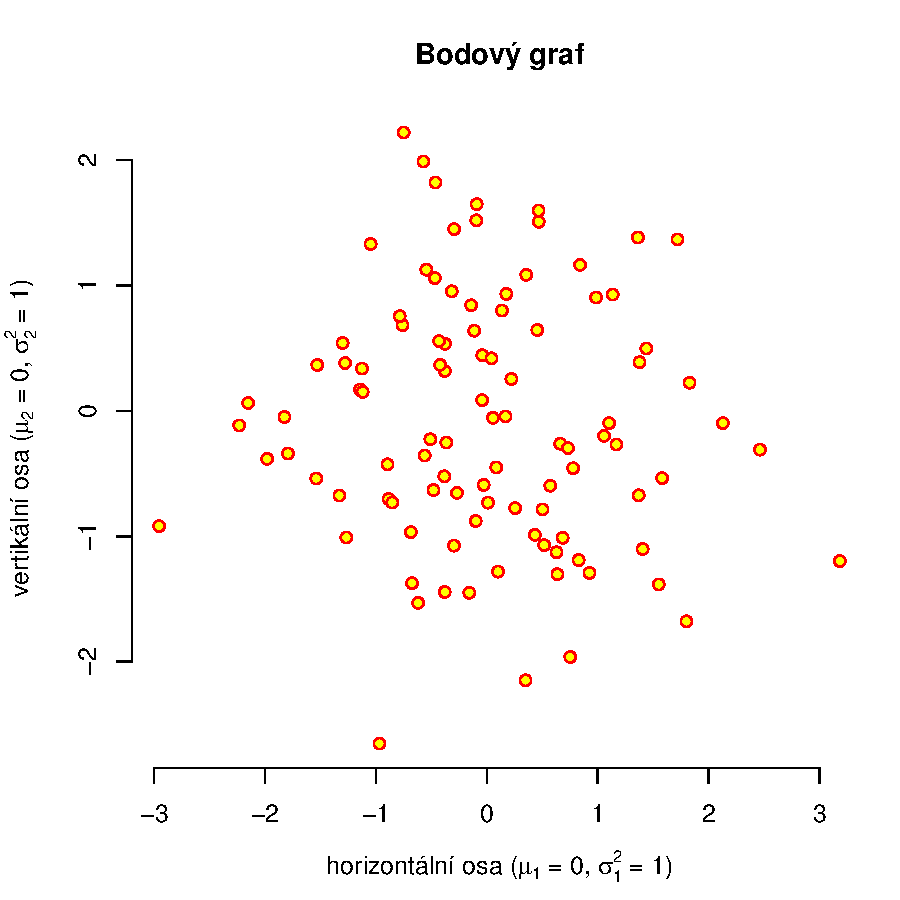
\includegraphics[height=0.8\textheight]{img/ukazka-obr01.pdf}
\end{frame}

\begin{frame}{Demo: showing something with comments}
\begin{columns}
\begin{column}{0.5\textwidth}
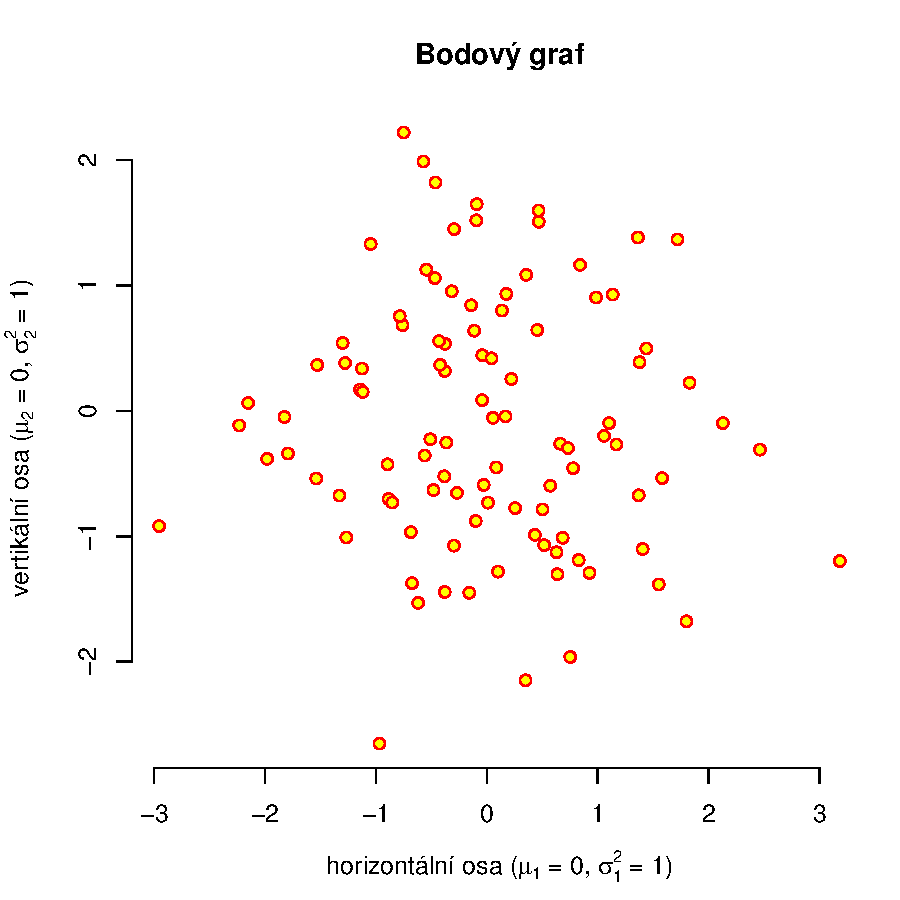
\includegraphics[width=\linewidth]{img/ukazka-obr01.pdf}
\end{column}
\begin{column}{0.5\textwidth}
How we arrived at this?
\begin{enumerate}
\item Generated the data
\item Plotted them
\item Used a very fine red marker to circle the points
\end{enumerate}

`Advantages' demo:

\begin{itemize}
\item[\color{green}\faCheck] Data is normal
\item[\color{red}\faTimes] Data is sparse
\item[\color{violet}\faQuestionCircle] What now?
\end{itemize}
\end{column}
\end{columns}
\end{frame}

% Ending frame is important -- in the rare case that you actually manage to
% finish the presentation on time, it avoids the embarassing seconds of silence
% between the time when you finish and the moment when committee detects that
% something is wrong and they should continue.
\begin{frame}[plain]
\centering
{\Large\bfseries Thank you for attention!}

You can try the results on GitHub: \\
\url{https://github.com/exaexa/simple-mff-slides}

\end{frame}
\end{document}
